\section{Gegen\"uberstellung der CST-Feldbilder der Kurzschlussanordnungen}
\label{sec:allfieldplots}
In diesem Abschnitt sind die Feldbilder abgebildet, die den Simulationsergebnissen aus CST entnommen wurden.
\begin{figure}[htb]
	\centering
	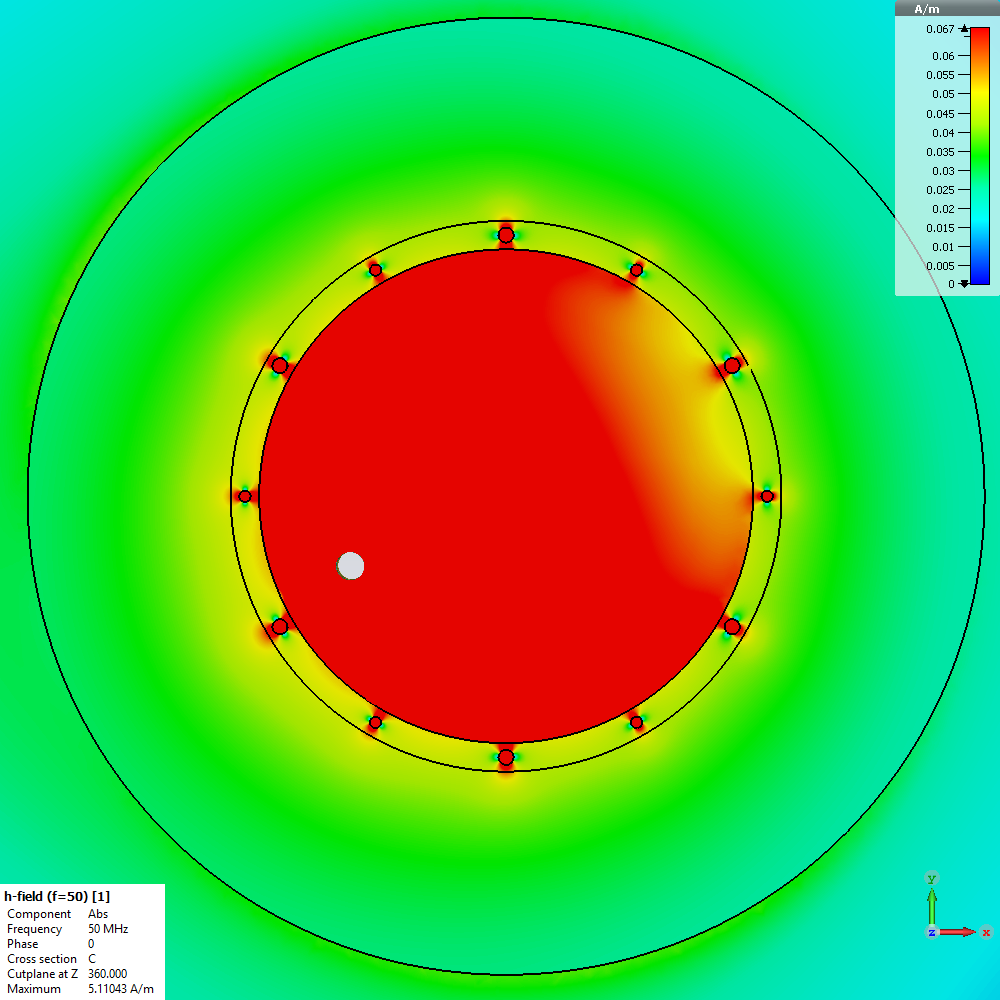
\includegraphics[width=0.5\textwidth]{Feldbilder/0KS}
	\caption{Feldbild des Ringkerns ohne Kurzschl\"usse.}
	\label{fig:field0ks}
\end{figure}

\begin{figure}[htb]
	\centering
	\subfloat[Breite $\SI{20}{\milli\meter}$]{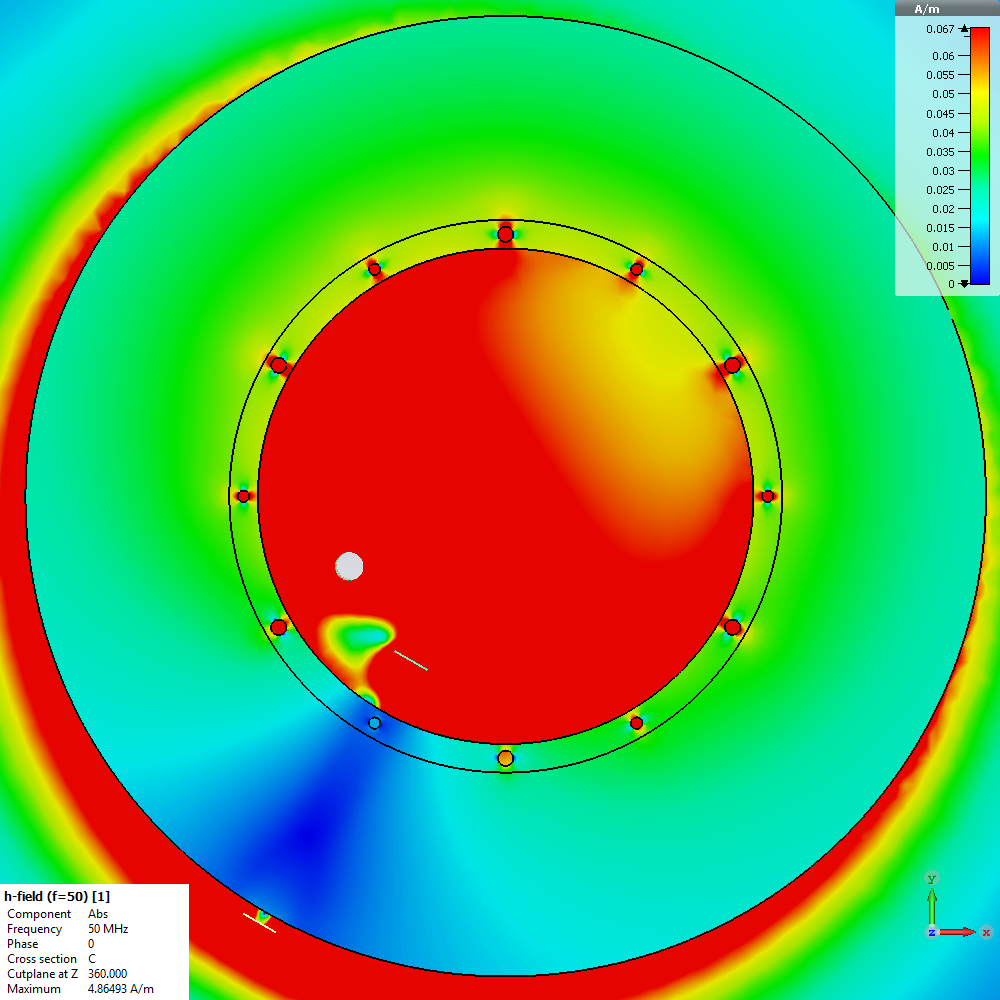
\includegraphics[width=0.33\textwidth]{Feldbilder/1KSb20}}
	\subfloat[$\SI{30}{\milli\meter}$]{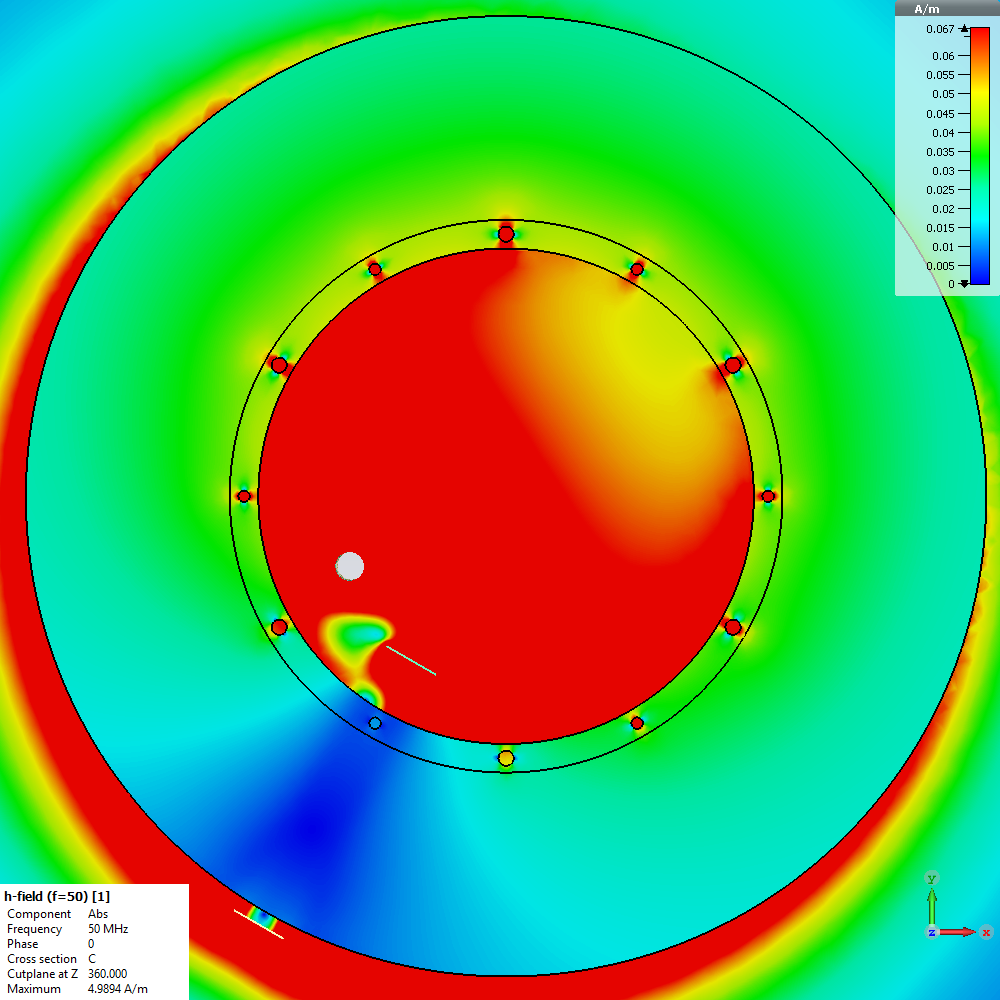
\includegraphics[width=0.33\textwidth]{Feldbilder/1KS}}
	\subfloat[Breite $\SI{50}{\milli\meter}$]{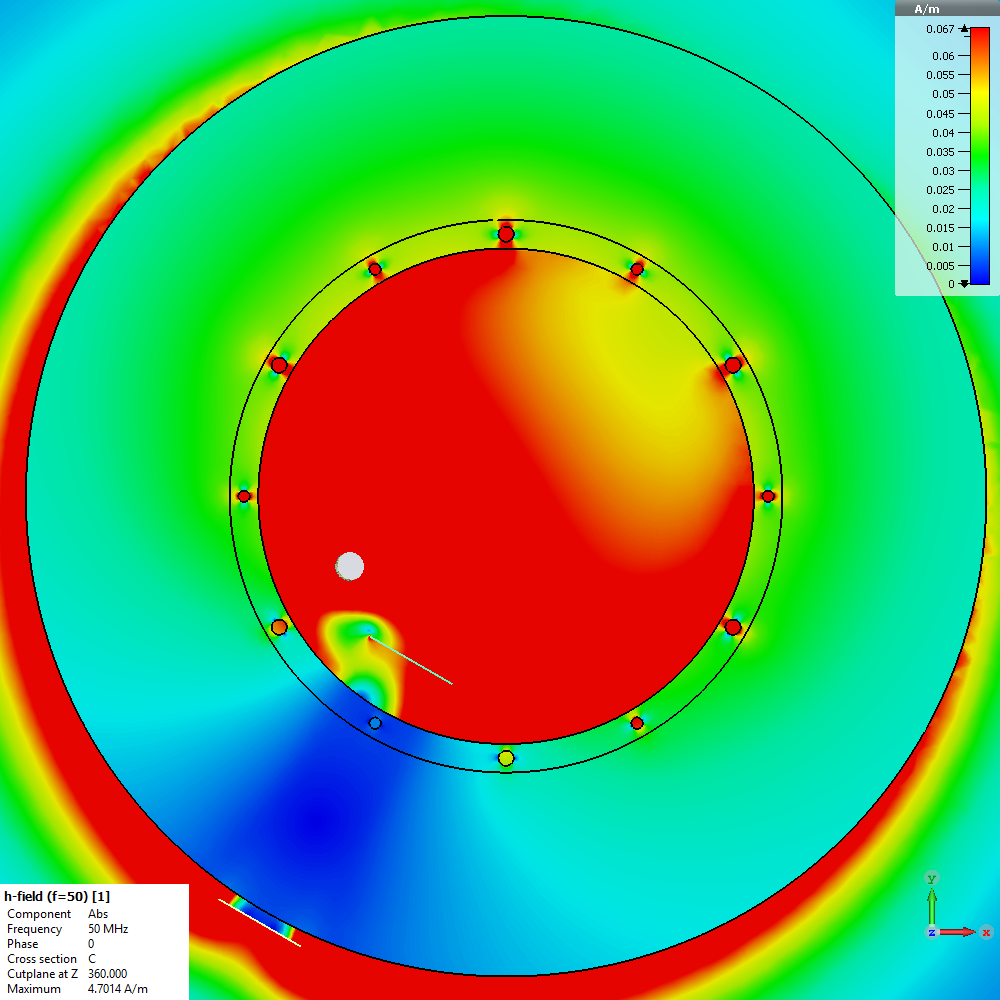
\includegraphics[width=0.33\textwidth]{Feldbilder/1KSb50}}
	\caption{Gegen\"uberstellung des Ringkerns mit jeweils einem Kurzschluss verschiedener Breiten und der Länge von $\SI{160}{\milli\meter}$.}
	\label{fig:field1ks}
\end{figure}

\begin{figure}[htb]
	\centering
	\subfloat[Breite $\SI{20}{\milli\meter}$]{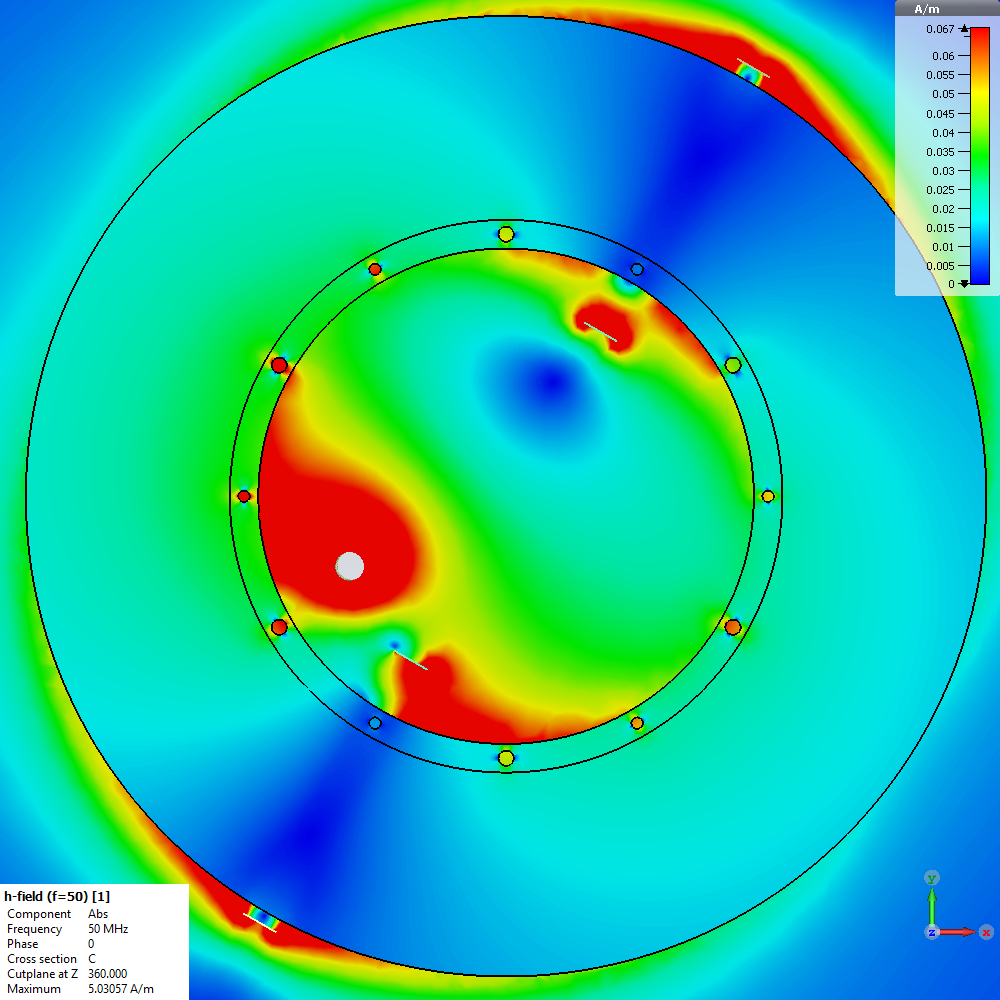
\includegraphics[width=0.33\textwidth]{Feldbilder/2KSb20}}
	\subfloat[Breite $\SI{30}{\milli\meter}$]{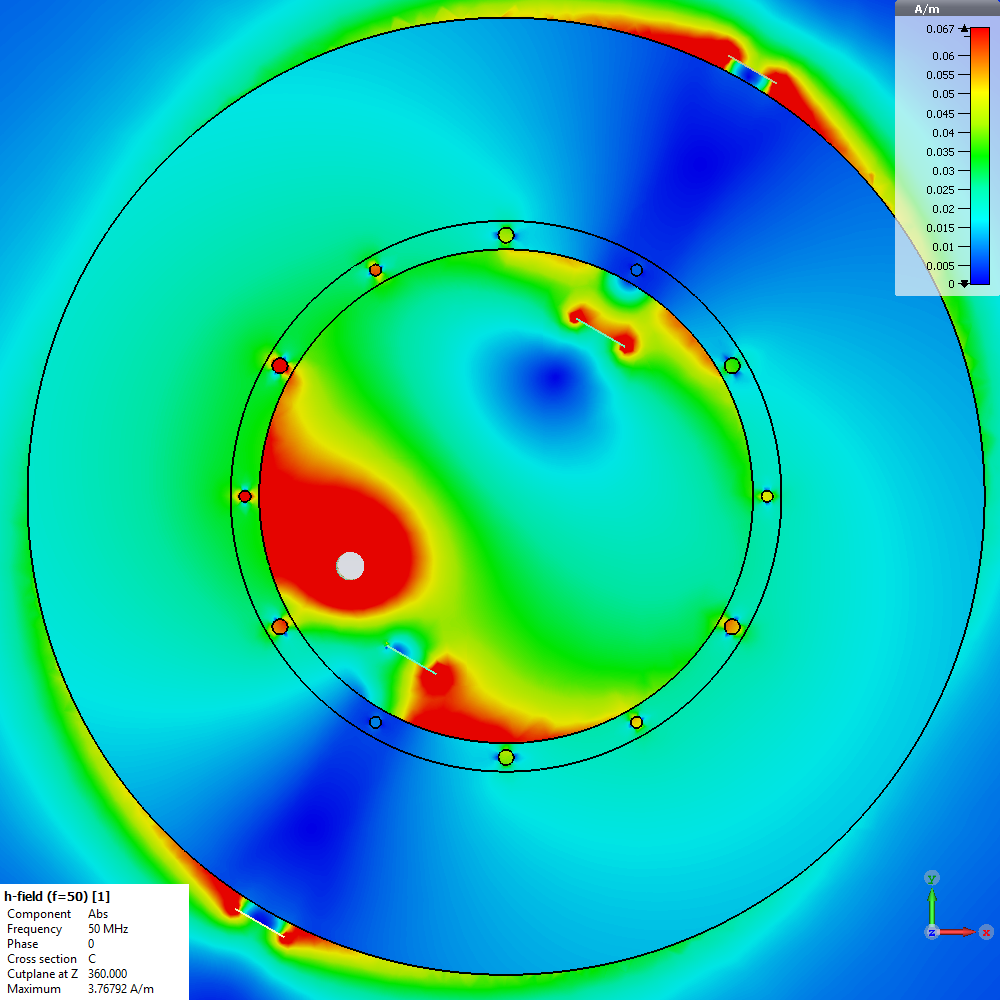
\includegraphics[width=0.33\textwidth]{Feldbilder/2KS}}
	\subfloat[Breite $\SI{50}{\milli\meter}$]{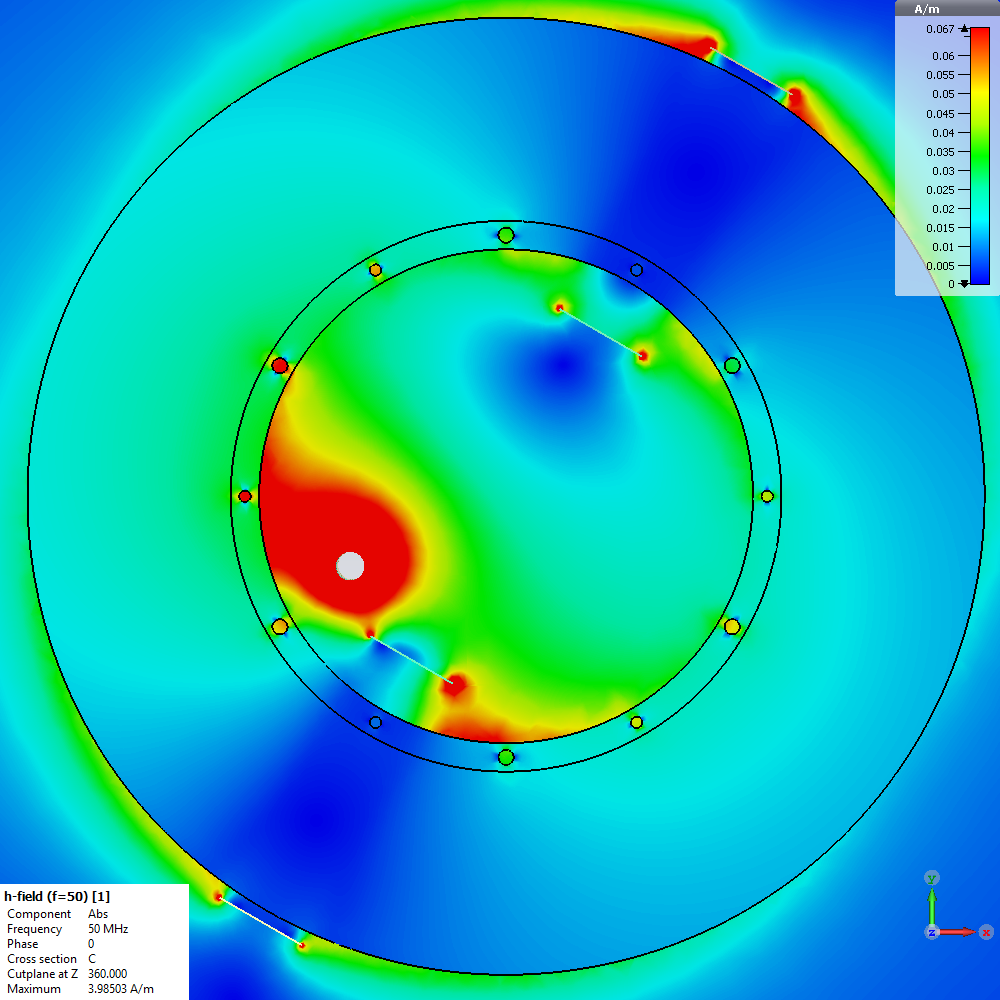
\includegraphics[width=0.33\textwidth]{Feldbilder/2KSb50}}
	\caption{Gegen\"uberstellung des Ringkerns mit jeweils zwei Kurzschl\"ussen verschiedener Breiten und der Länge von $\SI{160}{\milli\meter}$.}
	\label{fig:field2ks}
\end{figure}

\begin{figure}[htb]
	\centering
	\subfloat[3 Kurzschlüsse]{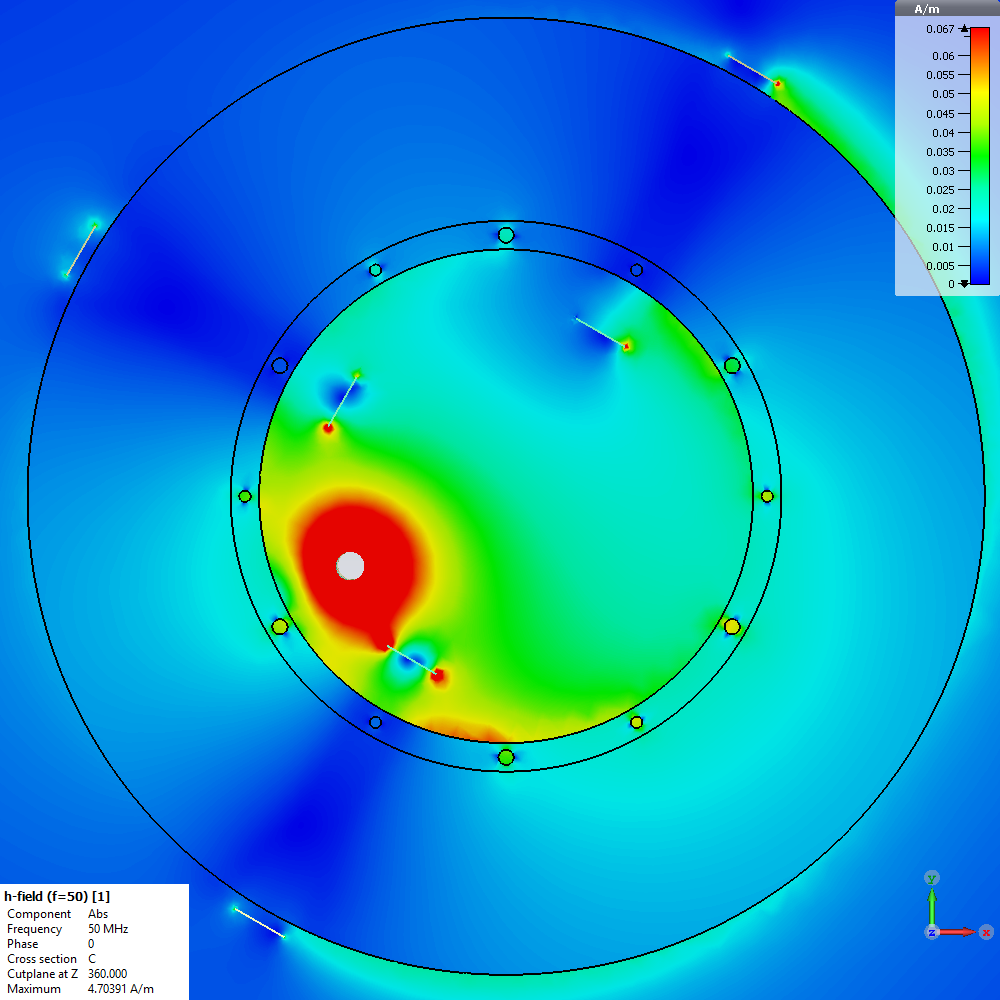
\includegraphics[width=0.33\textwidth]{Feldbilder/3KS}}
	\subfloat[4 Kurzschlüsse]{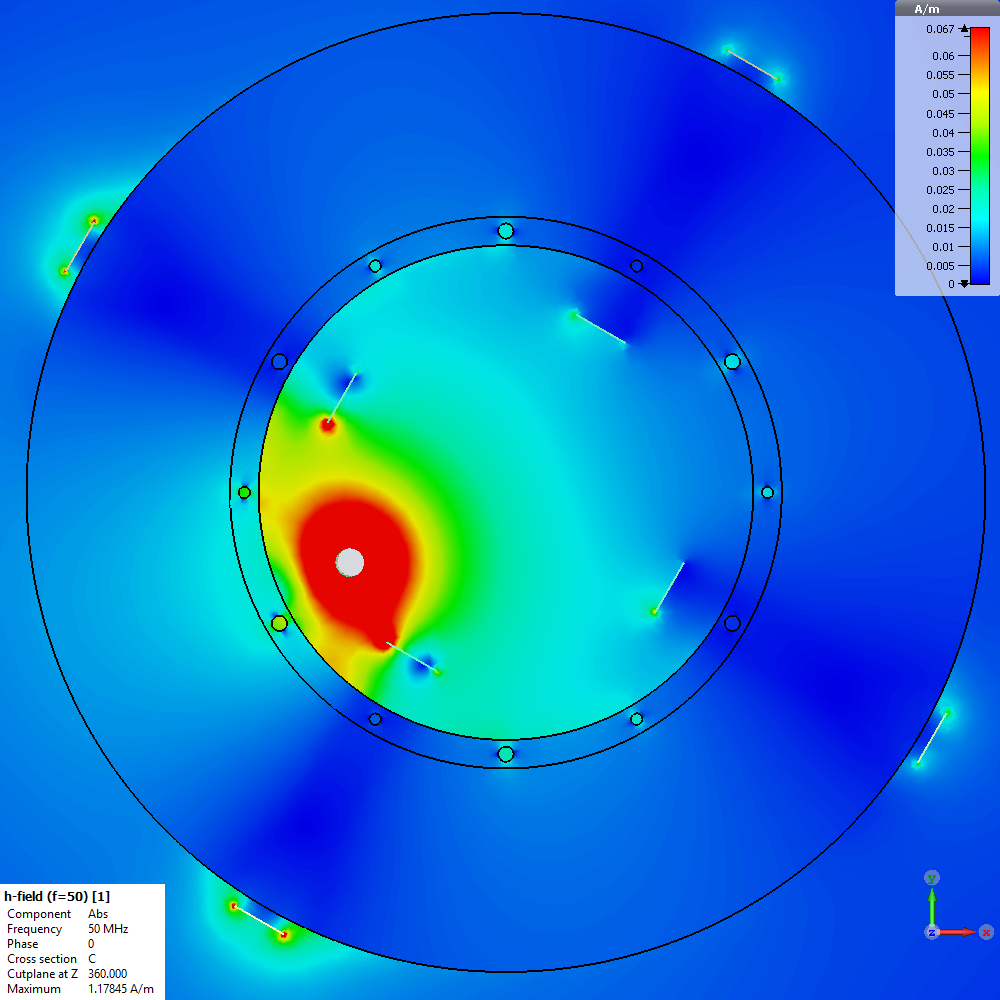
\includegraphics[width=0.33\textwidth]{Feldbilder/4KS}}
    \subfloat[5 Kurzschlüsse]{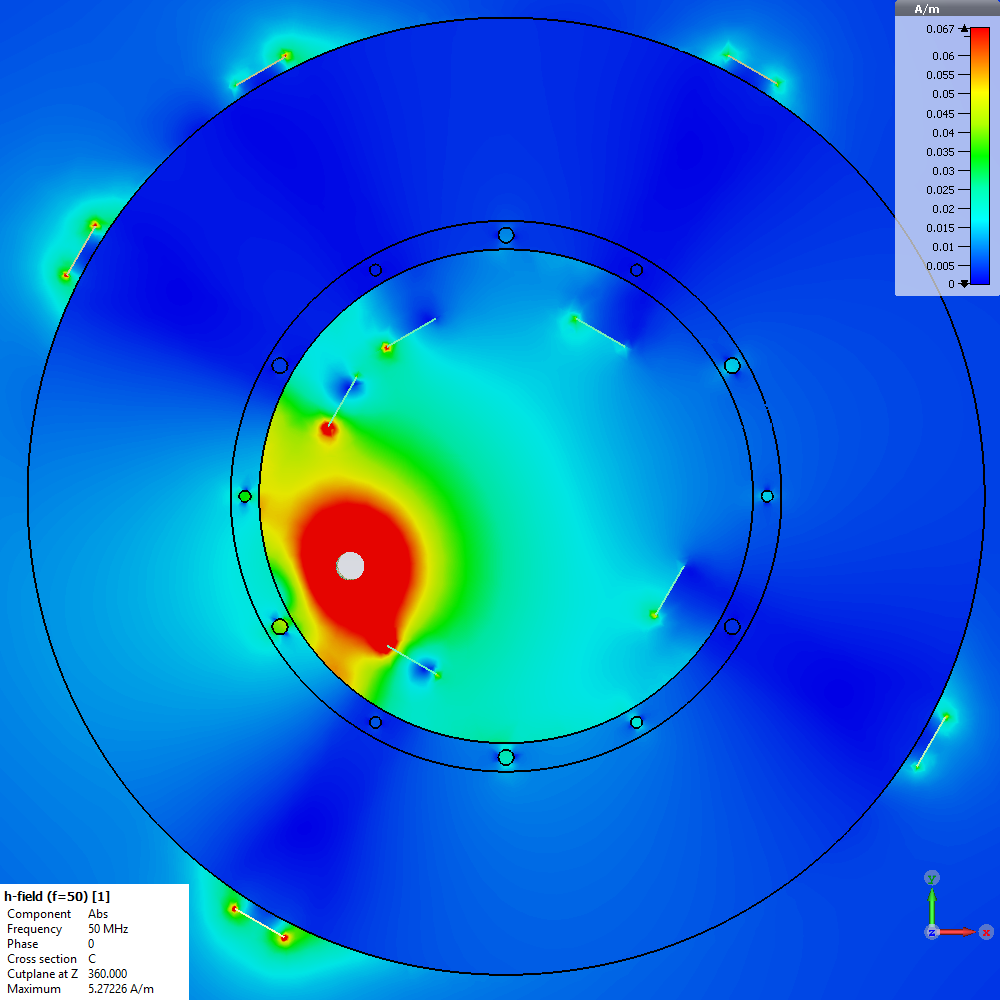
\includegraphics[width=0.33\textwidth]{Feldbilder/5KS}}\\
    \subfloat[6 Kurzschlüsse]{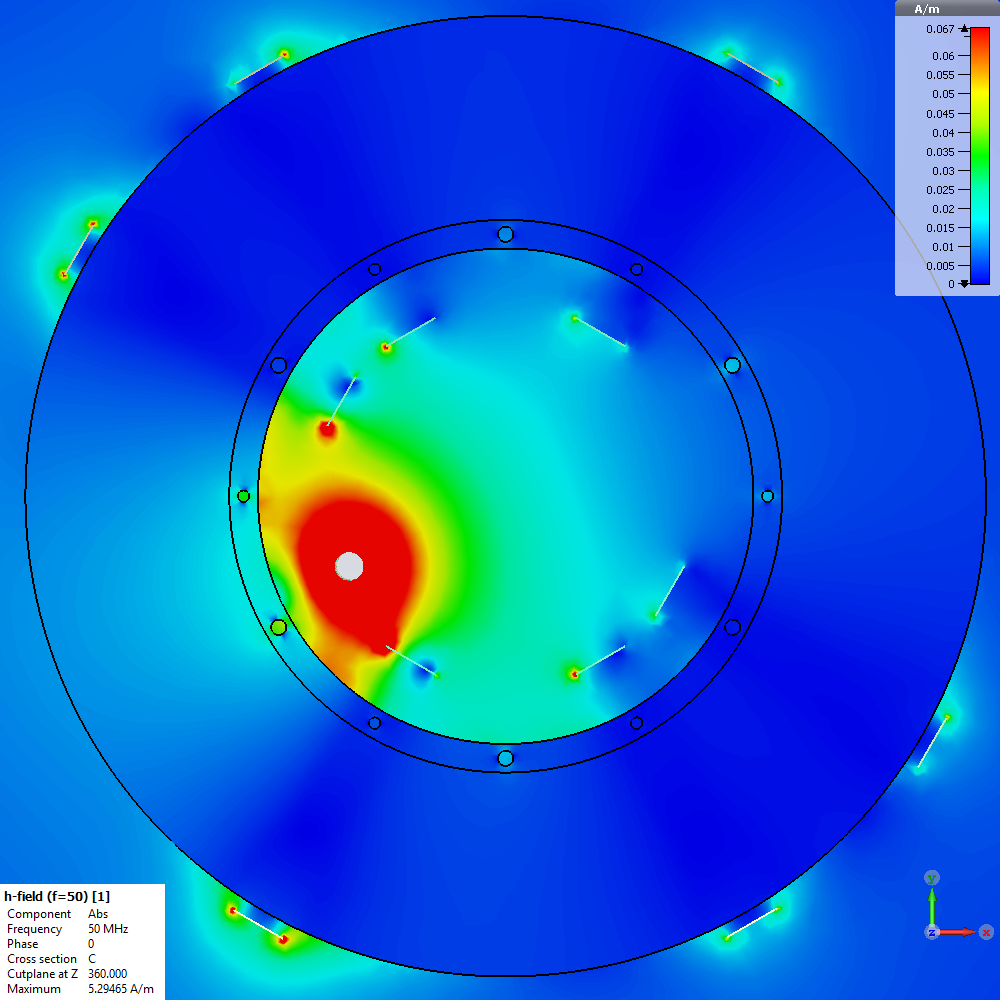
\includegraphics[width=0.33\textwidth]{Feldbilder/6KS}}
    \subfloat[7 Kurzschlüsse]{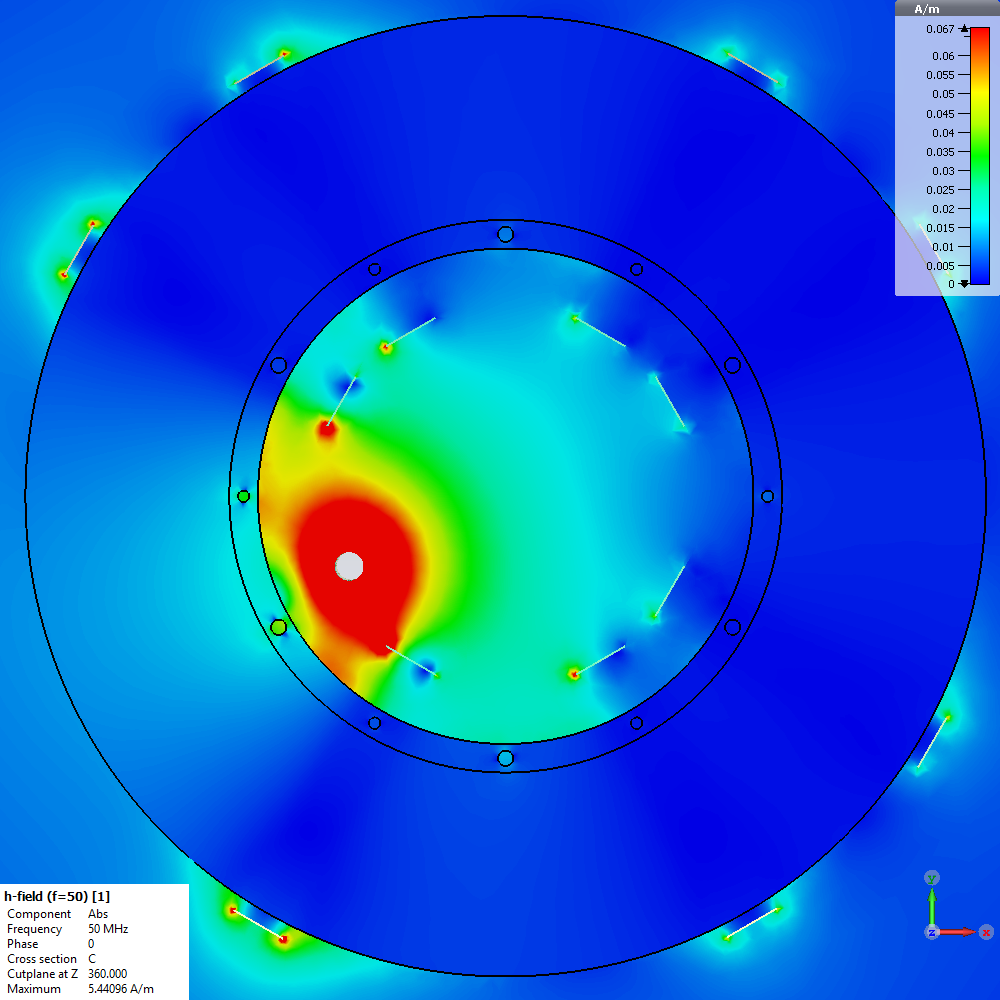
\includegraphics[width=0.33\textwidth]{Feldbilder/7KS}}
    \subfloat[8 Kurzschlüsse]{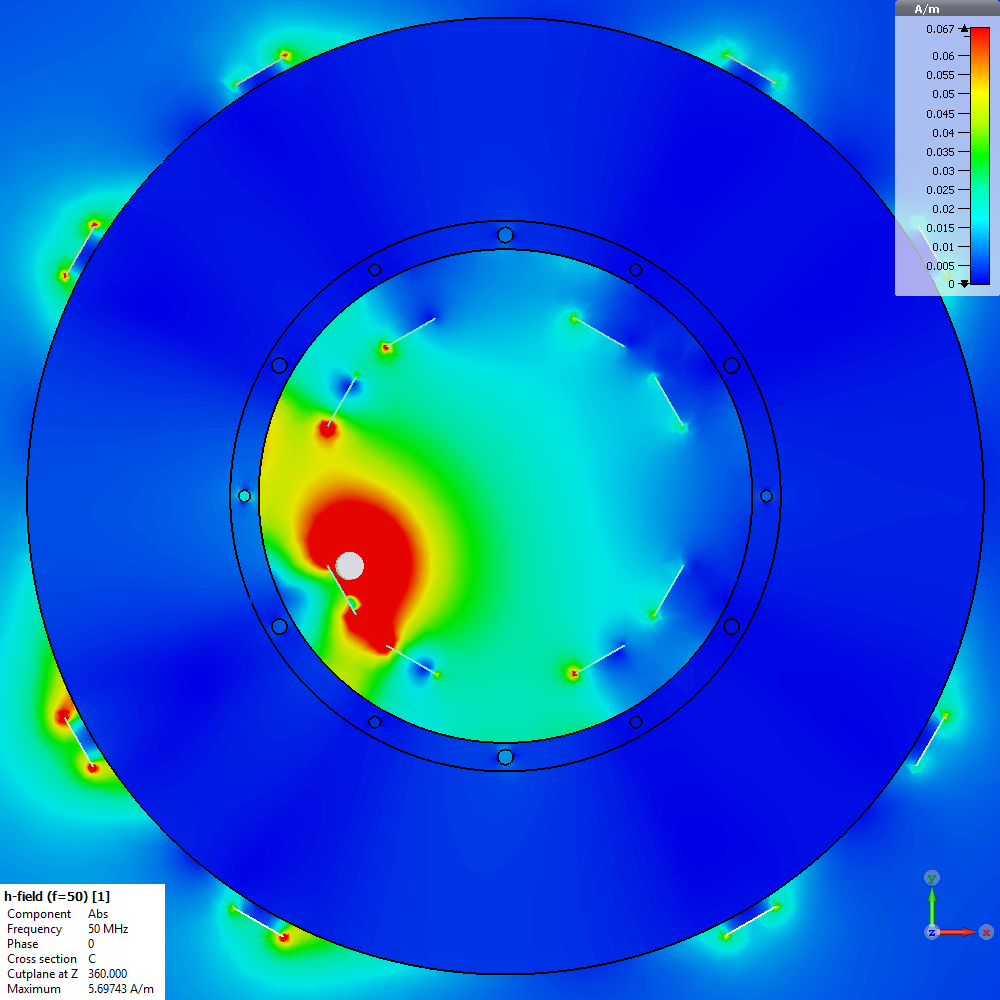
\includegraphics[width=0.33\textwidth]{Feldbilder/8KS}}
	\caption{Gegen\"uberstellung des Ringkerns mit drei bis acht Kurzschl\"ussen der Breite $\SI{30}{\milli\meter}$ und der Länge $\SI{160}{\milli\meter}$.}
	\label{fig:field3bis8ks}
\end{figure}
